\documentclass[11pt]{report}
\usepackage[utf8]{inputenc}
\usepackage[T1]{fontenc}
\usepackage[top=2.5cm, bottom=2.5cm, left=2cm, right=2cm]{geometry}
\usepackage{setspace}
\usepackage{graphicx}
\usepackage{float}
\usepackage{amsmath}
\usepackage{stmaryrd}
\usepackage{titlesec}
\usepackage{rotating}
\usepackage{alltt}
\usepackage{fancyvrb}
\usepackage{verbatimbox}
\usepackage{lipsum}
\usepackage{setspace}
\usepackage{tabto}
\usepackage{bussproofs}
\usepackage{caption}
\usepackage{subcaption}
\onehalfspacing
\titleformat{\chapter}[hang]{\bf\huge}{\thechapter}{2pc}{}

%-------------------------------------------------------
\let\oldabstract\abstract
\let\oldendabstract\endabstract
\makeatletter
\renewenvironment{abstract}
{\renewenvironment{quotation}%
               {\list{}{\addtolength{\leftmargin}{3em} % change this value to add or remove length to the the default
                        \listparindent 1.5em%
                        \itemindent    \listparindent%
                        \rightmargin   \leftmargin%
                        \parsep        \z@ \@plus\p@}%
                \item\relax}%
               {\endlist}%
\oldabstract}
{\oldendabstract}
\makeatother

\makeatletter
\newcommand{\verbatimfont}[1]{\renewcommand{\verbatim@font}{\normalfont#1}}
\makeatother

\begin{document}
\begin{center}

\includegraphics[scale = 1]{index.png}
\end{center}

\pagestyle{empty}
\vspace*{\stretch{8}}


\centerline{\textbf{\Huge Documentation}}
\bigbreak\bigbreak
\bigbreak\bigbreak

\centerline{ {\Large Estelle Alauzy}}
\vspace*{\stretch{1}}
\centerline{ {\Large  Chervin Amirkaveh}}


 \vfill
 \vspace*{\stretch{10}}
\centerline{\large June 2019}
\vspace*{\stretch{1}}






%%%%%%%%%%%%%%%%%%%%%%%%%%%%%%%%%%%%%%%%%%%%%%%%%%%%%%%%%%%%%%%%%%%%%%%%%%%%
%%%%%%%%%%%%%%%%%%%%%%%%%%%%%%%%%%%%%%%%%%%%%%%%%%%%%%%%%%%%%%%%%%%%%%%%%%%%

\newpage
\centerline{\textbf{\Huge Context}}
\vspace*{3pt}
\vspace*{20pt}

\tabto{1cm}Concurrency has become increasingly important in the last several years, increasing the need for verification tools for concurrent programs for languages such as Go, Erlang, and more. Although concurrent program equivalence has been studied for decades in the context of process algebras, a significant amount of theoretical results in this area have not reached the practice of software verification. 
\\ \\
\tabto{1cm}For example, one of the most well-established modelling language for concurrent, communicating systems is the pi-calculus. Researchers have used this language to develop some of the
most powerful techniques for program equivalence in a concurrent setting, which are based on (weak) bisimulation and its extensions (environmental bisimulation, up-to-context technique, up-to-* technique). However there is a distinct absence of tools for verifying the equivalence of pi-calculus terms.
\\ \\
\tabto{1cm}It is in this context that we have started the project to create a language that could be use as an intermediate language for a tool using a “bisimulation engine” back-end to prove the equivalence of programs.

\newpage
\centerline{\textbf{\Huge Description of the language}}
\vspace*{3pt}
\vspace*{20pt}
\tabto{1cm}First of all, this language is procedural meaning that procedures/functions are declared at top-level and can then be called anywhere in the program. This language contains basic and convenient features that you can find in most programming languages : basic types (integer, boolean, char, string), lists, 
tuples, local and global variables, functions declaration and call, different binary and unary operators for expressions, if-then-else, while and return instructions, ...
\\ \\
\tabto{1cm}However, what is making this language different from others is the integration of pi-calculus notions inside the language. Indeed, it is possible to declare channels as variables. Those channels can be used in different instructions : newChan, send and receive.
\begin{itemize}
\item \ ch = newChan(): create a new channel of the same type as the variable ch and assign it this new channel to it.
\item \ send(ch,e): send the expression e along the channel ch
\item \ v = receive(ch): receive an expression along the channel ch and assign it to the variable v
\end{itemize}

\tabto{1cm}The notion of input-guarded choice is also available in this language thanks to the instruction choose. The choose instructions allows you to use prefixes (new, send, receive, spawn, tau). The purpose of this instruction is the following: when the action of the prefix is possible, the action is made and the instructions corresponding to that prefix are executed after. In the case where actions of two different prefixes are possible at the same time, the program will choose one of them in a non-deterministic way.
\\ \\
\tabto{1cm} Finally, we have also added the instruction spawn to represent the parallelization of processes. Spawn can be seen as the "|" operator of the pi-calculus. It is important to note that spawn is not representing the immediate launch of a new thread. Indeed, when you code a sequence of spawn instructions, it's represents a simultaneous launch of all processes and not a sequential launch. The function and expression passed in arguments of the spawn instruction are used to create the new process.
\\ \\
\tabto{1cm} You will find below the grammar describing the language and a section about technical decisions that have impacted the language.

\newpage
\centerline{\textbf{\Huge Grammar : Backus-Naur form (BNF)}}
\vspace*{20 pt}
\vspace*{3pt}
\begin{Verbatim}[fontfamily=textsf]
Program ::= TypeDecla Program
            | FuncDecla Program
            | VariableDeclaGlobal Program
            | FuncDecla CallMain
            | VariableDeclaGlobal CallMain
\end{Verbatim}
\vspace*{3pt}

\begin{verbnobox}[\normalfont]
FuncDecla ::= func FuncType name (Parameters) Body
\end{verbnobox}
\vspace*{3pt}

\begin{verbnobox}[\normalfont]
TypeDecla ::= type name = Typ
\end{verbnobox}
\vspace*{3pt}

\begin{verbnobox}[\normalfont]
Parameters ::= Typ identifier | Typ identifier , Parameters
\end{verbnobox}
\vspace*{3pt}

\begin{verbnobox}[\normalfont]
Body ::= { Instruction } | { def VariableDeclas in Instruction }
\end{verbnobox}
\vspace*{3pt}

\begin{verbnobox}[\normalfont]
VariableDeclaGlobal ::= Typ identifier = Value | Typ identifier = (ValueSeq)
\end{verbnobox}
\vspace*{3pt}

\begin{verbnobox}[\normalfont]
VariableDecla ::= Typ identifier
\end{verbnobox}
\vspace*{3pt}

\begin{verbnobox}[\normalfont]
VariableDeclas ::= VariableDecla 
                    | VariableDeclas ; 
                    | VariableDecla ; VariableDeclas
\end{verbnobox}
\vspace*{3pt}

\begin{verbnobox}[\normalfont]
Instruction ::= ; Instruction
               |
               | Bintruction 
               | Binstruction ; Instruction
\end{verbnobox}
\vspace*{3pt}

\begin{verbnobox}[\normalfont]
Binstruction ::= Expression = Expression 
                 | Expression = name ( ExpressionSeq )
                 | name ( ExpressionSeq )
                 | Expression = receive ( identifier )
                 | send ( identifier , Expression )
                 | if ( Expression ) { Instruction } else { Instruction }
                 | while ( Expression ) { Instruction }
                 | choose { Choices }
                 | spawn name ( ExpressionSeq )
                 | Expression = newChan()
                 | return
                 | return Expression
                 | return name (ExpressionSeq)
\end{verbnobox}
\vspace*{3pt}

\begin{verbnobox}[\normalfont]
Choices ::= Prefix -> { Instruction } Choices | Prefix -> { Instruction }
\end{verbnobox}
\vspace*{3pt}

\begin{verbnobox}[\normalfont]
Prefix ::= | tau
         | | send ( identifier , Expression )
         | | Expression = receive ( identifier )
         | | Expression = newChan()
         | | spawn name ( ExpressionSeq )
\end{verbnobox}
\vspace*{3pt}

\begin{verbnobox}[\normalfont]
Expression ::= - Expression
               | not Expression
               | head ( Expression )
               | tail ( Expression )
               | odd ( Expression )
               | even ( Expression )
               | fst ( Expression )
               | snd ( Expression )
               | Expression + Expression
               | Expression - Expression
               | Expression || Expression
               | Expression * Expression
               | Expression / Expression
               | Expression && Expression
               | Expression == Expression
               | Expression != Expression 
               | Expression < Expression
               | Expression > Expression
               | get(Expression,Expression)
               | if ( Expression ) { Expression } else { Expression }
               | ( ExpressionSeq )
               | Value
               | identifier
\end{verbnobox}
\vspace*{3pt}

\begin{verbnobox}[\normalfont]
ExpressionSeq ::= Expression | Expression , ExpressionSeq
\end{verbnobox}
\vspace*{3pt}

\begin{verbnobox}[\normalfont]
Constant ::= integer
             | ' char '
             | ""
             | " string "
             | true
             | false
\end{verbnobox}
\vspace*{3pt}

\begin{verbnobox}[\normalfont]
Value ::= Constant | [ ValueSeq ] | []
\end{verbnobox}
\vspace*{3pt}

\begin{verbnobox}[\normalfont]
ValueSeq ::= Value | Value , ValueSeq
\end{verbnobox}
\vspace*{3pt}

\begin{verbnobox}[\normalfont]
Typ ::= int
      | boolean
      | string
      | char
      | channel Typ
      | list [ Types ]
      | ( Types )
      | identifier
\end{verbnobox}
\vspace*{3pt}

\begin{verbnobox}[\normalfont]
Types ::= Typ | Typ , Types
\end{verbnobox}
\vspace*{3pt}

\begin{verbnobox}[\normalfont]
FuncType ::= void | Typ
\end{verbnobox}
\vspace*{3pt}

\begin{verbnobox}[\normalfont]
CallMain ::= start name ( ExpressionSeq )
\end{verbnobox}
\vspace*{3pt}

\newpage
\centerline{\textbf{\Huge Technical choices for the parser}}
\vspace*{3pt}
\vspace*{10pt}
\tabto{0cm} {\Large \textbf{Conflicts resolution}}
\\ \\ 
\tabto{1cm} In order to remove ambiguities in our grammar and so resolve shift/reduce conflicts we have added some rules. It is important to note that in our grammar the majority of our conflicts refer to binary operators.  \\ \\
By declaring precedence and associative rules for all tokens involved in the conflicts, this force derivations to be done in a particular way.
\\ \\ 
\tabto{2cm} \textbf{Associativity}
\\ \\
\tabto{1cm} The first way to make unambiguous our grammar is by establishing associative rules for an operator "op". Theses rules determines how to interpret the operator's repetition: if "x op y op z" must be considered as "(x op y) op z" or "x op (y op z)". \\ \\
There are three different ways to specify them. 
\begin{itemize}
\item \%right:  makes the operator right-associative
\item \%left: makes the operator left-associative
\item \%nonassoc: makes the association incorrect, i.e.: "x op y op z" will be considered as a syntax error.
\end{itemize}
We have decided that the operators: $*$, $+$, $-$, $/$, $=$, $\ne$, $\&\&$ and $||$ are left-associative and that for the operators $>$ and $<$ the association is incorrect.
\\ \\ \\
\tabto{2cm} \textbf{Precedence}
\\ \\
\tabto{1cm} The second way to make unambiguous our grammar is by imposing the precedence of one operator over the other. The relative precedence between the different operators is defined by the order in which they are declared. The first declared has the lowest precedence and so the last declared has the highest precedence. We have chosen the order of the precedence in way that the different operators respect the arithmetic logic.
\\ \\
\newpage
We have also used semi-colons to resolve conflicts. \\ \\
\tabto{2cm} \textbf{Semi-colon} \\ \\
\tabto{1cm}Semi-colons allow to separate instructions from each other and so that avoid shift-reduce conflicts at the level of the assign and return operators. It also makes our grammar more resistant and so easier for someone to add new instructions without causing conflicts. \\ \\
\tabto{1cm} In our grammar, the semicolon should not be interpreted as an end of line indication but simply as a separator between variable declarations or instructions:
\begin{itemize}
\item For instructions: a semicolon sequence is translated by the parser as a sequence of empty instructions.
\item For variable declarations: this is not possible, however it is possible to end the declarations with a semicolon without causing an error syntax but it makes no sense in our grammar. We have implemented this to avoid mistakes due to the use of other languages.
\end{itemize}

\newpage
\centerline{\textbf{\Huge Type Grammar}}
\vspace*{3pt}
\vspace*{20pt}
We have created types that simplify our grammar and so allow us to perform a more efficient type checking. We have separated the types for expressions and instructions.

\tabto{0cm} {\Large \textbf{Simplified type for Expressions}}

\tabto{0cm}The possible types for an expression of this language are described by the following syntax:
\\ \\
\centerline{$\tau \rightarrow int \ | \ bool \ | \ string \ | \ char \ | \ void$} \\
\tabto{6,6cm}$ channel( \tau) \ | \ channel $ \\
\tabto{6,6cm}$ list(\tau) \ | \ list $ \\
\tabto{6,6cm}$ ( \tau \ list) \ | \ tuple $ \\
\tabto{6,6cm}$ namedtype(string)$ \\
\tabto{6,6cm}$ Error $

\tabto{0cm} {\Large \textbf{Simplified type for Instructions}}

\tabto{0cm}The possible types for an instruction of this language are described by the following syntax:
\\ \\
\centerline{$OK \ | \ OK_t(\tau)$}

\tabto{0cm} {\Large \textbf{Environments}}

\tabto{0cm} Before checking the types of the expressions and instructions, we create 2 environments:
\begin{itemize}
\item The type environment: composed of the different declared types (named types)
\item The variable environment composed of all defined global variables and defined functions
\end{itemize}
So, the environments only concern what is declared at the top level.\\

In order to create these 2 environments, it is necessary to verify that each declared element is well formed before adding it to its corresponding environment.\\ \\
Concerning the type environment, being well-formed means: 
The name used is unique in the environment, the other types used to declare this type are well-formed types i.e. other named types defined above or a basic type defined in our language (int, string, char...) and the declared type is recursive only if it is a channel type\\ \\ \\
Concerning the variable environment, first it is  necessary to distinguish functions and variables.
\begin{itemize}
    \item  For variables, being well-formed means: The name used is unique in the environment and the variables's type is a well formed type
    \item For functions, being well-formed means: The name used is unique in the environment, the function return's type is a well formed type, and the parameters are well-formed (all parameters type are well formed and each parameter has an unique name)
\end{itemize}
Finally, we have to check that the function used in the start function is declared.

\newpage
\centerline{\textbf{\Huge Type Rules}}
\vspace*{35pt}

\tabto{1cm} {\Large \textsc{Type rules for expressions}}

\vspace*{20pt}

\tabto{0cm} {\large \textbf{Unary Operator}}
\begin{prooftree}
\AxiomC{$\Gamma_t ; \ \Gamma_v \vdash e : \tau $}
\AxiomC{$op \ : \tau \rightarrow \tau'$ }
\BinaryInfC{$\Gamma_t ; \ \Gamma_v \vdash op \ e : \tau' $}
\end{prooftree}

\tabto{0cm} {\large \textbf{Binary Operator}}
\begin{prooftree}
\AxiomC{$\Gamma_t ; \ \Gamma_v ; \vdash e_1: \tau_1 $}
\AxiomC{$\Gamma_t ; \ \Gamma_v \vdash e_2 : \tau_2$}
\AxiomC{$op \ : \tau_1 \times \tau_2 \rightarrow \tau$ }
\TrinaryInfC{$\Gamma_t ; \ \Gamma_v ; \vdash e_1 \ op \ e_2 : \tau $}
\end{prooftree}

\tabto{0cm} {\large \textbf{Condition Expression}}
\begin{prooftree}
\AxiomC{$\Gamma_t ; \ \Gamma_v \vdash e_1 : bool $}
\AxiomC{$\Gamma_t ; \ \ \Gamma_v \vdash e_2 : \tau $}
\AxiomC{$\Gamma_t ; \ \Gamma_v \vdash e_3 : \tau $}
\TrinaryInfC{$\Gamma_t ; \ \Gamma_v \vdash if \ (e_1) \ then \ \{ e_2\} \ else \ \{e_3\} : \tau $}
\end{prooftree}

\tabto{0cm} {\large \textbf{Tuple}}
\begin{prooftree}
\AxiomC{$\Gamma_t ; \ \Gamma_v \vdash e_1 : \tau_1$}
\AxiomC{$\Gamma_t ; \ \Gamma_v \vdash e_2 : \tau_2 $}
\AxiomC{$\ldots$}
\AxiomC{$\Gamma_t ; \ \Gamma_v \vdash e_n : \tau_n $}
\QuaternaryInfC{$\Gamma_t ; \ \Gamma_v \vdash (e_1,e_2,\ldots,e_n) : (\tau_1 \times \tau_2 \times \ldots \times \tau_n)$}
\end{prooftree}

\tabto{0cm} {\large \textbf{List of Values}}
\begin{prooftree}
\AxiomC{$\Gamma_t ; \ \Gamma_v \vdash e_1 : \tau$}
\AxiomC{$\Gamma_t ; \ \Gamma_v \vdash e_2 : \tau$}
\AxiomC{$\ldots$}
\AxiomC{$\Gamma_t ; \ \Gamma_v \vdash e_n : \tau$}
\QuaternaryInfC{$\Gamma_t ; \ \Gamma_v \vdash [e_1,e_2,\ldots,e_n] : list [\tau]$}
\end{prooftree}

\tabto{0cm} {\large \textbf{Identifier}}
\begin{prooftree}
\AxiomC{$ x : \tau \in \Gamma_v$}
\UnaryInfC{$\Gamma_t ; \ \Gamma_v \vdash x : \tau$}
\end{prooftree}

\newpage

\tabto{1cm} {\Large \textsc{Type rules for instructions}}
\vspace*{20pt}

\tabto{0cm} {\large \textbf{Sequence of Instructions}}
\begin{prooftree}
\AxiomC{$\Gamma_t ; \ \Gamma_v \vdash i_1 : OK$}
\AxiomC{$\Gamma_t ; \ \Gamma_v \vdash i_2 : \tau $}
\BinaryInfC{$\Gamma_t ; \ \Gamma_v \vdash i_1 \ ; \ i_2 :  OK_t(\tau) $}
\end{prooftree}

\begin{prooftree}
\AxiomC{$\Gamma_t ; \ \Gamma_v \vdash i_1 : OK$}
\AxiomC{$\Gamma_t ; \ \Gamma_v \vdash i_2 : OK $}
\BinaryInfC{$\Gamma_t ; \ \Gamma_v \vdash i_1 \ ; \ i_2 :  OK) $}
\end{prooftree}

\begin{prooftree}
\AxiomC{$\Gamma_t ; \ \Gamma_v \vdash i_1 : \tau$}
\AxiomC{$\Gamma_t ; \ \Gamma_v \vdash i_2 : \tau $}
\BinaryInfC{$\Gamma_t ; \ \Gamma_v \vdash i_1 \ ; \ i_2 :  OK_t(\tau) $}
\end{prooftree}

\tabto{0cm} {\large \textbf{Assignment Instruction}}
\begin{prooftree}
\AxiomC{$\Gamma_t ; \ \Gamma_v ; \vdash a : \tau_a $}
\AxiomC{$\Gamma_t ; \ \Gamma_v \vdash e : \tau_e$}
\AxiomC{$ \tau_a = \tau_e $}
\TrinaryInfC{$\Gamma_t ; \ \Gamma_v ; \vdash a = e : OK $}
\end{prooftree}

\tabto{0cm} {\large \textbf{Function Call with return}}
\begin{prooftree}
\AxiomC{$\Gamma_t ; \ \Gamma_v \vdash a : \tau_2 $}
\AxiomC{$\Gamma_t ; \ \Gamma_v \vdash e_2 : \tau_1 \rightarrow \tau_2 $}
\AxiomC{$\Gamma_t ; \ \Gamma_v \vdash e_3 : \tau_1 $}
\TrinaryInfC{$\Gamma_t ; \ \Gamma_v \vdash a = e_2 (e_3) : OK $}
\end{prooftree}

\tabto{0cm} {\large \textbf{Function Call without return}}
\begin{prooftree}
\AxiomC{$\Gamma_t ; \ \Gamma_v \vdash e_1 : \tau_1 \rightarrow void$}
\AxiomC{$\Gamma_t ; \ \Gamma_v \vdash e_2 : \tau_1 $}
\BinaryInfC{$\Gamma_t ; \ \Gamma_v \vdash e_1(e_2) : OK $}
\end{prooftree}

\tabto{0cm} {\large \textbf{Receive Instruction}}
\begin{prooftree}
\AxiomC{$\Gamma_t ; \ \Gamma_v \vdash c : chan \ \tau $}
\AxiomC{$\Gamma_t ; \ \Gamma_v \vdash a : \tau $}
\BinaryInfC{$\Gamma_t ; \ \Gamma_v \vdash a = receive(c) : OK $}
\end{prooftree}

\tabto{0cm} {\large \textbf{Send Instruction}}
\begin{prooftree}
\AxiomC{$\Gamma_t ; \ \Gamma_v \vdash c : chan \ \tau $}
\AxiomC{$\Gamma_t ; \ \Gamma_v \vdash e : \tau $}
\BinaryInfC{$\Gamma_t ; \ \Gamma_v \vdash send(c,e) : OK $}
\end{prooftree}

\tabto{0cm} {\large \textbf{Condition Instruction}}
\begin{prooftree}
\AxiomC{$\Gamma_t ; \ \Gamma_v \vdash e : bool $}
\AxiomC{$\Gamma_t ; \ \ \Gamma_v \vdash i_1 : OK $}
\AxiomC{$\Gamma_t ; \ \Gamma_v \vdash i_2 : OK $}
\TrinaryInfC{$\Gamma_t ; \ \Gamma_v \vdash if \ (e) \ then \ \{i_1\} \ else \ \{i_2\} : OK $}
\end{prooftree}
\vspace*{1pt}
\begin{prooftree}
\AxiomC{$\Gamma_t ; \ \Gamma_v \vdash e : bool $}
\AxiomC{$\Gamma_t ; \ \ \Gamma_v \vdash i_1 : OK_t(\tau) $}
\AxiomC{$\Gamma_t ; \ \Gamma_v \vdash i_2 : OK_t(\tau) $}
\TrinaryInfC{$\Gamma_t ; \ \Gamma_v \vdash if \ (e) \ then \ \{i_1\} \ else \ \{i_2\} : OK_t(\tau) $}
\end{prooftree}

\tabto{0cm} {\large \textbf{While Instruction}}
\begin{prooftree}
\AxiomC{$\Gamma_t ; \ \Gamma_v \vdash e : bool$}
\AxiomC{$\Gamma_t ; \ \Gamma_v \vdash i : OK $}
\BinaryInfC{$\Gamma_t ; \ \Gamma_v \vdash while(e) \ \{ i \} : OK $}
\end{prooftree}
\vspace*{1pt}
\begin{prooftree}
\AxiomC{$\Gamma_t ; \ \Gamma_v \vdash e : bool$}
\AxiomC{$\Gamma_t ; \ \Gamma_v \vdash i : OK_t(\tau) $}
\BinaryInfC{$\Gamma_t ; \ \Gamma_v \vdash while(e) \ \{ i \} : OK_t(\tau) $}
\end{prooftree}

\tabto{0cm} {\large \textbf{Choose Instruction}}
\begin{prooftree}
\AxiomC{$\Gamma_t ; \ \Gamma_v \vdash p_1 : OK \ \ldots \ \Gamma_t ; \ \Gamma_v \vdash p_n : OK $}
\AxiomC{$\Gamma_t ; \ \Gamma_v \vdash i_1 : OK \ \ldots \ \Gamma_t ; \ \Gamma_v \vdash i_n : OK $}
\BinaryInfC{$\Gamma_t ; \ \Gamma_v \vdash Choose \{ \ \ | \ p_1 -> i_1 \ \ | \ \ldots \ | \ p_n -> i_n \ \ \} : OK $}
\end{prooftree}
\vspace*{1pt}
\begin{prooftree}
\AxiomC{$\Gamma_t ; \ \Gamma_v \vdash p_1 : OK \ \ldots \ \Gamma_t ; \ \Gamma_v \vdash p_n : OK $}
\AxiomC{$\Gamma_t ; \ \Gamma_v \vdash i_1 : OK_t(\tau) \ \ldots \ \Gamma_t ; \ \Gamma_v \vdash i_n : OK_t(\tau) $}
\BinaryInfC{$\Gamma_t ; \ \Gamma_v \vdash Choose \{ \ \ | \ p_1 -> i_1 \ \ | \ \ldots \ | \ p_n -> i_n \ \ \} : OK_t(\tau) $}
\end{prooftree}

\tabto{0cm} {\large \textbf{Spawn Instruction}}
\begin{prooftree}
\AxiomC{$\Gamma_t ; \ \Gamma_v \vdash e_1 : \tau_1 \rightarrow void$}
\AxiomC{$\Gamma_t ; \ \Gamma_v \vdash e_2 : \tau_1 $}
\BinaryInfC{$\Gamma_t ; \ \Gamma_v \vdash spawn \ e_1(e_2) : OK $}
\end{prooftree}

\tabto{0cm} {\large \textbf{NewChan Instruction}}
\begin{prooftree}
\AxiomC{$\Gamma_t ; \ \Gamma_v \vdash a : chan \ \tau $}
\UnaryInfC{$\Gamma_t ; \ \Gamma_v \vdash a = newChan() : OK $}
\end{prooftree}

\tabto{0cm} {\large \textbf{Return void}}
\begin{prooftree}
\AxiomC{$ $}
\UnaryInfC{$\Gamma_t ; \ \Gamma_v \vdash return \ OK $}
\end{prooftree}

\tabto{0cm} {\large \textbf{Return Expression }}
\begin{prooftree}
\AxiomC{$\Gamma_t ; \ \Gamma_v \vdash e : \tau$}
\UnaryInfC{$\Gamma_t ; \ \Gamma_v \vdash return \ e \ : OK_t(\tau) $}
\end{prooftree}

\tabto{0cm} {\large \textbf{Return Function }}
\begin{prooftree}
\AxiomC{$\Gamma_t ; \ \Gamma_v \vdash e_1 : \tau_1 \rightarrow \tau_2$}
\AxiomC{$\Gamma_t ; \ \Gamma_v \vdash e_2 : \tau_1 $}
\BinaryInfC{$\Gamma_t ; \ \Gamma_v \vdash return \ e_1(e_2) : OK_t\{\tau_2\} $}
\end{prooftree}

\newpage

\tabto{0cm} {\large \textbf{Function Declaration}}
\begin{prooftree}
\AxiomC{$wf(\Gamma_{extended} = \{\Gamma_t ; \ \Gamma_v; \ \overrightarrow{\tau \ \ x} ; \ \overrightarrow{\tau^\prime \ \ y})$}
\AxiomC{$\Gamma_{extended} \vdash i : OK_t(\tau_f) $}
\BinaryInfC{$\Gamma_t ; \ \Gamma_v \vdash func \ \tau_f \ n  (\overrightarrow{\tau \ \ x}) \ \{def \  \overrightarrow{\tau^\prime \ \ y} \ in \ i \} \ : OK_t(\tau_f) $}
\end{prooftree}
\vspace*{1pt}
\begin{prooftree}
\AxiomC{$wf(\Gamma_{extended} = \{\Gamma_t ; \ \Gamma_v; \ \overrightarrow{\tau \ \ x} ; \ \overrightarrow{\tau^\prime \ \ y}\})$}
\AxiomC{$\Gamma_{extended} \vdash i : OK $}
\BinaryInfC{$\Gamma_t ; \ \Gamma_v \vdash func \ void \ n  (\overrightarrow{\tau \ \ x}) \ \{def \  \overrightarrow{\tau^\prime \ \ y}\} \ in \ i \} \ : OK $}
\end{prooftree}


\newpage
\centerline{\textbf{\Huge Semantic Rules (Small-step semantics)}}
\vspace*{3pt}
\vspace*{20pt}

\tabto{1cm} {\Large \textsc{Semantics rules for expressions}}
\vspace*{20pt}

\tabto{0cm} {\large \textbf{Binary Operator}}
\begin{prooftree}
\AxiomC{$G;S \vdash e_1 \Downarrow  v_1 $}
\AxiomC{$G;S \vdash e_2 \Downarrow  v_2$}
\BinaryInfC{$G;S \vdash e_1 \ op \ e_2 \Downarrow v_1 \ op \ v_2 $}
\end{prooftree}

\tabto{0cm} {\large \textbf{Unary Operator}}
\begin{prooftree}
\AxiomC{$G;S \vdash e \Downarrow  v $}
\UnaryInfC{$G;S \vdash op \ e \Downarrow v $}
\end{prooftree}

\tabto{0cm} {\large \textbf{Condition Expression}}
\begin{prooftree}
\AxiomC{$G;S \vdash e_1 \Downarrow true $}
\AxiomC{$G;S \vdash e_2 \Downarrow v $}
\BinaryInfC{$G;S \vdash if \ e_1 \ then \ e_2 \ else \ e_3  \Downarrow v $}
\end{prooftree}
\vspace*{1pt}
\begin{prooftree}
\AxiomC{$G;S \vdash e_1 \Downarrow false $}
\AxiomC{$G;S \vdash e_3 \Downarrow v $}
\BinaryInfC{$G;S \vdash if \ e_1 \ then \ e_2 \ else \ e_3  \Downarrow v $}
\end{prooftree}


\tabto{0cm} {\large \textbf{Tuple}}
\begin{prooftree}
\AxiomC{$G;S \vdash e_1 \Downarrow v_1 $}
\AxiomC{$G;S \vdash e_2 \Downarrow v_2 $}
\AxiomC{$\ldots$}
\AxiomC{$G;S \vdash e_n \Downarrow v_n $}
\QuaternaryInfC{$G;S \vdash (e_1,e_2,\ldots,e_n) \Downarrow (v_1, v_2, \ldots, v_n)$}
\end{prooftree}

\tabto{0cm} {\large \textbf{Value}}
\begin{prooftree}
\AxiomC{ }
\UnaryInfC{$G;S \vdash v \Downarrow v $}
\end{prooftree}

\tabto{0cm} {\large \textbf{Identifier}}
\begin{prooftree}
\AxiomC{ }
\UnaryInfC{$G;S \vdash n \Downarrow lookup \ n \ in \ S $}
\end{prooftree}

\newpage
\tabto{1cm} {\Large \textsc{Semantics rules for instructions}}
\vspace*{20pt}

\tabto{0cm} {\large \textbf{Assignment}}
\begin{prooftree}
\AxiomC{$G;S \vdash e \Downarrow v $}
\UnaryInfC{$G;S;E \vdash a = e \rightarrow_{\beta} G;S::[a \mapsto v];E \vdash noop$}
\end{prooftree}

\tabto{0cm} {\large \textbf{Condition Instruction}}
\begin{prooftree}
\AxiomC{$G;S \vdash e \Downarrow true $}
\UnaryInfC{$G;S;E \vdash  if \ e \ then \ i_1 \ else \ i_2 \rightarrow_{\beta} G;S;E \vdash i_1$}
\end{prooftree}
\vspace*{1pt}
\begin{prooftree}
\AxiomC{$G;S \vdash e \Downarrow false $}
\UnaryInfC{$G;S;E \vdash  if \ e \ then \ i_1 \ else \ i_2 \rightarrow_{\beta} G;S;E \vdash i_2$}
\end{prooftree}

\tabto{0cm} {\large \textbf{Function Call with return}}
\begin{prooftree}
\AxiomC{$G;S \vdash \overrightarrow{e} \Downarrow \overrightarrow{v}$}
\AxiomC{$ G(f) = (\lambda \overrightarrow{x}.i,S_f)$}
\BinaryInfC{$G;S;E \vdash a = f (\overrightarrow{e}) \rightarrow_{\beta} G;G::[\overrightarrow{x} \mapsto \overrightarrow{v}]::S_f;(S;a=[.])::E \vdash i$}
\end{prooftree}

\tabto{0cm} {\large \textbf{Function Call without return}}
\begin{prooftree}
\AxiomC{$G;S \vdash \overrightarrow{e} \Downarrow \overrightarrow{v}$}
\AxiomC{$ G(f) = (\lambda \overrightarrow{x}.i,S_f)$}
\BinaryInfC{$G;S;E \vdash f (\overrightarrow{e}) \rightarrow_{\beta} G;G::[\overrightarrow{x} \mapsto \overrightarrow{v}]::S_f;(S;void)::E \vdash i$}
\end{prooftree}

\tabto{0cm} {\large \textbf{While Instruction}}
\begin{prooftree}
\AxiomC{$G;S \vdash e \Downarrow true $}
\UnaryInfC{$G;S;E \vdash  while(e) \ \{i\} \rightarrow_{\beta} G;S;E \vdash i; while(e) \ \{i\}$}
\end{prooftree}
\vspace*{1pt}
\begin{prooftree}
\AxiomC{$G;S \vdash e \Downarrow false $}
\UnaryInfC{$G;S;E \vdash  while(e) \ \{i\} \rightarrow_{\beta} G;S;E \vdash noop$}
\end{prooftree}

\tabto{0cm} {\large \textbf{Return void}}
\begin{prooftree}
\AxiomC{$ $}
\UnaryInfC{$G;S;(S';void)::E \vdash return \rightarrow_{\beta} G;S';E \vdash noop$}
\end{prooftree}

\tabto{0cm} {\large \textbf{Return Function ?}}


\tabto{0cm} {\large \textbf{Assign of a function return}}
\begin{prooftree}
\AxiomC{$ $}
\UnaryInfC{$G;S;(S';a=[.])::E \vdash return \ v \rightarrow_{\beta} G;S';[a \mapsto v]::E \vdash noop$}
\end{prooftree}

\tabto{0cm} {\large \textbf{Return Break}}
\begin{prooftree}
\AxiomC{$ $}
\UnaryInfC{$G;S;(noop;seqi)::E \vdash return \ e \rightarrow_{\beta} G;S;E \vdash return \ e$}
\end{prooftree}

\tabto{0cm} {\large \textbf{Sequence of Instructions}}
\begin{prooftree}
\AxiomC{$ $}
\UnaryInfC{$G;S;E \vdash i ; seqi \rightarrow_{\beta} G;S;(noop;seqi)::E \vdash i$}
\end{prooftree}

\tabto{0cm} {\large \textbf{Noop}}
\begin{prooftree}
\AxiomC{$ $}
\UnaryInfC{$G;S;(noop;seqi)::E \vdash noop \rightarrow_{\beta} G;S;E \vdash seqi$}
\end{prooftree}

\tabto{0cm} $\Delta = G;S;E$

\tabto{0cm} {\large \textbf{NewChan Instruction}}
\begin{prooftree}
\AxiomC{$ $}
\UnaryInfC{$ N;\Delta \vdash a = newChan() \rightarrow_{\beta} N \oplus {n};\Delta[a \mapsto n] \vdash noop $}
\end{prooftree}

\tabto{0cm} {\large \textbf{Receive Instruction}}
\begin{prooftree}
\AxiomC{$N;S \vdash ch \Downarrow n$}
\UnaryInfC{$N;\Delta \vdash a = receive(ch) \underset{n?v}{\longrightarrow} N;\Delta[a \mapsto v] \vdash noop $}
\end{prooftree}

\tabto{0cm} {\large \textbf{Send Instruction}}
\begin{prooftree}
\AxiomC{$N;S \vdash ch \Downarrow n$}
\AxiomC{$N;S \vdash e \Downarrow v$}
\BinaryInfC{$N;\Delta \vdash send(ch,e) \underset{n!v}{\longrightarrow} N;\Delta \vdash noop$}
\end{prooftree}

\tabto{0cm} {\large \textbf{Choose Instruction}}
\begin{prooftree}
\AxiomC{$ $}
\UnaryInfC{$N;\Delta \vdash choose \{ \overrightarrow{ \ p \longrightarrow i \ } \} \rightarrow N;G;S;(noop;i_k)::E \vdash p_k $}
\end{prooftree}

\newpage
\centerline{\textbf{\Huge Semantic Rules (Big-Step Semantics)}}
\vspace*{3pt}
\vspace*{20pt}

\tabto{1cm} {\Large \textsc{Semantics rules for expressions}}
\vspace*{20pt}

\tabto{0cm} {\large \textbf{Binary Operator}}
\begin{prooftree}
\AxiomC{$s \vdash e_1 \Downarrow  v_1 $}
\AxiomC{$s \vdash e_2 \Downarrow  v_2$}
\BinaryInfC{$s \vdash e_1 \ op \ e_2 \Downarrow v_1 \ op \ v_2 $}
\end{prooftree}

\tabto{0cm} {\large \textbf{Unary Operator}}
\begin{prooftree}
\AxiomC{$s \vdash e \Downarrow  v $}
\UnaryInfC{$s \vdash op \ e \Downarrow v $}
\end{prooftree}

\tabto{0cm} {\large \textbf{Condition Expression}}
\begin{prooftree}
\AxiomC{$s \vdash e_1 \Downarrow true $}
\AxiomC{$s \vdash e_2 \Downarrow v $}
\BinaryInfC{$s \vdash if \ e_1 \ then \ e_2 \ else \ e_3  \Downarrow v $}
\end{prooftree}
\vspace*{1pt}
\begin{prooftree}
\AxiomC{$s \vdash e_1 \Downarrow false $}
\AxiomC{$s \vdash e_3 \Downarrow v $}
\BinaryInfC{$s \vdash if \ e_1 \ then \ e_2 \ else \ e_3  \Downarrow v $}
\end{prooftree}


\tabto{0cm} {\large \textbf{Tuple}}
\begin{prooftree}
\AxiomC{$s \vdash e_1 \Downarrow v_1 $}
\AxiomC{$s \vdash e_2 \Downarrow v_2 $}
\AxiomC{$\ldots$}
\AxiomC{$s \vdash e_n \Downarrow v_n $}
\QuaternaryInfC{$s \vdash (e_1,e_2,\ldots,e_n) \Downarrow (v_1, v_2, \ldots, v_n)$}
\end{prooftree}

\tabto{0cm} {\large \textbf{Value}}
\begin{prooftree}
\AxiomC{ }
\UnaryInfC{$s \vdash v \Downarrow v $}
\end{prooftree}

\tabto{0cm} {\large \textbf{Identifier}}
\begin{prooftree}
\AxiomC{ }
\UnaryInfC{$s \vdash n \Downarrow lookup \ n \ in \ s $}
\end{prooftree}

\newpage
\tabto{1cm} {\Large \textsc{Semantics rules for instructions}}
\vspace*{20pt}

\tabto{0cm} {\large \textbf{Assignment}}
\begin{prooftree}
\AxiomC{$s \vdash e \Downarrow v $}
\UnaryInfC{$s \vdash a = e \Downarrow \emptyset, s[a \mapsto v] $}
\end{prooftree}

\tabto{0cm} {\large \textbf{Condition Instruction}}
\begin{prooftree}
\AxiomC{$s_1 \vdash e \Downarrow true $}
\AxiomC{$s_1 \vdash i_1 \Downarrow \emptyset, s_2$}
\BinaryInfC{$s_1 \vdash if \ e \ then \ i_1 \ else \ i_2  \Downarrow \emptyset, s_2 $}
\end{prooftree}
\vspace*{1pt}
\begin{prooftree}
\AxiomC{$s_1 \vdash e \Downarrow true $}
\AxiomC{$s_1 \vdash i_1 \Downarrow v, s_2$}
\BinaryInfC{$s_1 \vdash if \ e \ then \ i_1 \ else \ i_2  \Downarrow v, s_2 $}
\end{prooftree}
\vspace*{1pt}
\begin{prooftree}
\AxiomC{$s_1 \vdash e \Downarrow false $}
\AxiomC{$s_1 \vdash i_2 \Downarrow \emptyset, s_2$}
\BinaryInfC{$s_1 \vdash if \ e \ then \ i_1 \ else \ i_2  \Downarrow \emptyset, s_2 $}
\end{prooftree}
\vspace*{1pt}
\begin{prooftree}
\AxiomC{$s_1 \vdash e \Downarrow false $}
\AxiomC{$s_1 \vdash i_2 \Downarrow v, s_2$}
\BinaryInfC{$s_1 \vdash if \ e \ then \ i_1 \ else \ i_2  \Downarrow v, s_2 $}
\end{prooftree}


\tabto{0cm} {\large \textbf{Function Call with return}}
\begin{prooftree}
\AxiomC{$s \vdash f \Downarrow (\lambda x.i),(s::s_l) $}
\AxiomC{$s \vdash e \Downarrow v_1 $}
\AxiomC{$(s::s_l)::[x \mapsto v_1] \vdash i \Downarrow v_2, s$}
\TrinaryInfC{$s \vdash a = f (e) \Downarrow s[a \mapsto v_2]$}
\end{prooftree}

\tabto{0cm} {\large \textbf{Function Call without return}}
\begin{prooftree}
\AxiomC{$s \vdash f \Downarrow (\lambda x.i),(s::s_l) $}
\AxiomC{$s \vdash e \Downarrow v $}
\AxiomC{$(s::s_l)::[x \mapsto v] \vdash i \Downarrow \emptyset, s$}
\TrinaryInfC{$s_1 \vdash f (e) \Downarrow \emptyset, s$}
\end{prooftree}

\tabto{0cm} {\large \textbf{While Instruction}}
\begin{prooftree}
\AxiomC{$s_1 \vdash e \Downarrow true $}
\AxiomC{$s_1 \vdash i \Downarrow \emptyset, s_2$}
\BinaryInfC{$s_1 \vdash while(e) \ \{i\} \Downarrow  while(e) \ \{i\},s_2 $}
\end{prooftree}
\vspace*{1pt}
\begin{prooftree}
\AxiomC{$s \vdash e \Downarrow false $}
\UnaryInfC{$s \vdash while(e) \ \{i\} \Downarrow \emptyset, s $}
\end{prooftree}
\vspace*{1pt}
\begin{prooftree}
\AxiomC{$s_1 \vdash e \Downarrow true $}
\AxiomC{$s_1 \vdash i \Downarrow v,s_2 $}
\BinaryInfC{$s_1 \vdash while(e) \ \{i\} \Downarrow  v,s_2 $}
\end{prooftree}


\tabto{0cm} {\large \textbf{Return void}}
\begin{prooftree}
\AxiomC{$ $}
\UnaryInfC{$s \vdash return \Downarrow \emptyset $}
\end{prooftree}

\tabto{0cm} {\large \textbf{Return Function }}
\begin{prooftree}
\AxiomC{$s_1 \vdash e \Downarrow v,s_2 $}
\UnaryInfC{$s_1 \vdash return \ e \Downarrow v,s_2 $}
\end{prooftree}

\tabto{0cm} {\large \textbf{Return Expression }}
\begin{prooftree}
\AxiomC{$s_1 \vdash e \Downarrow v,s_2 $}
\UnaryInfC{$s_1 \vdash return \ e \Downarrow v,s_2 $}
\end{prooftree}

\tabto{0cm} {\large \textbf{Sequence of Instructions}}
\begin{prooftree}
\AxiomC{$s_1 \vdash i_1 \Downarrow \emptyset, s_2$}
\AxiomC{$s_2 \vdash i_2 \Downarrow \emptyset, s_3 $}
\BinaryInfC{$s_1 \vdash i_1 \ ; \ i_2 \Downarrow \emptyset, s_3 $}
\end{prooftree}
\vspace*{1pt}
\begin{prooftree}
\AxiomC{$s_1 \vdash i_1 \Downarrow \emptyset, s_2$}
\AxiomC{$s_2 \vdash i_2 \Downarrow v, s_3 $}
\BinaryInfC{$s_1 \vdash i_1 \ ; \ i_2 \Downarrow v,s_3 $}
\end{prooftree}
\vspace*{1pt}
\begin{prooftree}
\AxiomC{$s_1 \vdash i_1 \Downarrow v,s_2$}
\UnaryInfC{$s_1 \vdash i_1 \ ; \ i_2 \Downarrow v,s_2 $}
\end{prooftree}

\tabto{0cm} {\large \textbf{Local Variable Declaration}}
\begin{prooftree}
\AxiomC{$x \notin dom(s)$}
\UnaryInfC{$s \vdash type \ x \Downarrow s::[x \mapsto v_{type}]$}
\end{prooftree}

\tabto{0cm} {\large \textbf{Global Variable Declaration}}
\begin{prooftree}
\AxiomC{$x \notin dom(s)$}
\UnaryInfC{$s \vdash type \ x = v \Downarrow s::[x \mapsto v]$}
\end{prooftree}

\newpage
\centerline{\textbf{\Huge Examples}}
\vspace*{3pt}
\vspace*{20pt}
\tabto{0cm} {\Large \textbf{Mobiles phones (example-10)}}
\vspace*{3pt}
\\
This example is highly inspired by the "mobile phones system" example - page 82 - of the book: \\
\textit{Communicating and mobile systems: the $\pi$-calculus} by Robin Milner 

\begin{center}
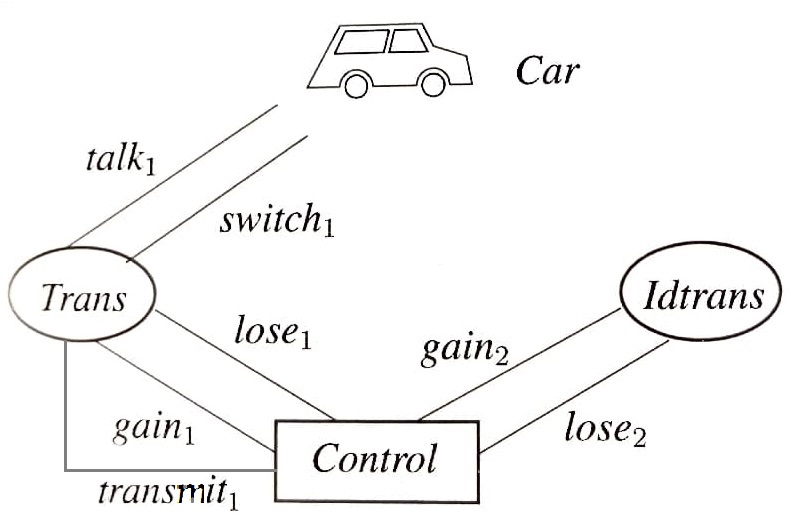
\includegraphics[scale = 0.5]{mobile-phone-system.jpg}
\end{center}
In our example, we made some modifications compared to the original example from the book. To allow the control to know when it needs to act we add an other channel between Control and Trans named transmit1. This channel transmit the message received by Trans from Car. This message is an integer which represents the position of the car. We arbitrarily decide at which position the links between the Trans and the car must be switched to the other trans : Idtrans. So, when the position is greater than the threshold the Control tells to Trans to lose the car and to IdTrans to gain the car.

\vspace*{15pt}
\tabto{0cm} {\Large \textbf{Buffer of size n (example-11)}}
\vspace*{3pt}
\\
In this example, we consider a buffer of n cells. First, in $\pi$-calculus the definition of a buffer cell by :
$B(l,r) = l(x).C \langle x,l,r \rangle$ and $C(x,l,r) = \bar{r} \langle x \rangle .B \langle l,r \rangle$

\begin{center}
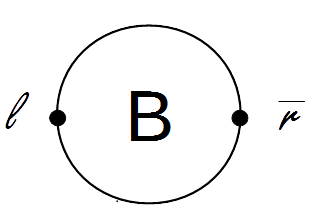
\includegraphics[scale = 0.25]{BufferCell.png}
\end{center}
So to create a buffer of size n, we make a chain of n buffer cells. This system is defined by linking :
$B^{(n)} = \overbrace{B^{ \frown} \ldots ^{\frown} B}^{\text{n times}}$

\begin{center}
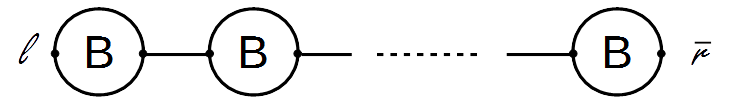
\includegraphics[scale = 0.4]{Buffern.png}
\end{center}

\newpage

\tabto{0cm} {\Large \textbf{Chemical reaction (example-12)}}
\vspace*{3pt}
\\
In this example we are trying to simulate the following chemical reaction : \\
$K + Na + 2Cl = K^+ + Na^+ + 2Cl^-$ \\
For each type of atoms, there are dedicated channels on which they liberate or capture an electron. The ionization and deionization process are associated with the receive and send instruction. An atom can capture an electron only if an another atom is ready to liberate one and vice-versa. In our example, the thermochemical laws are not respected because the reaction can occur in both ways at anytime.  

\begin{figure}[!h]
    \centering
    \begin{subfigure}[b]{0.3\textwidth}
        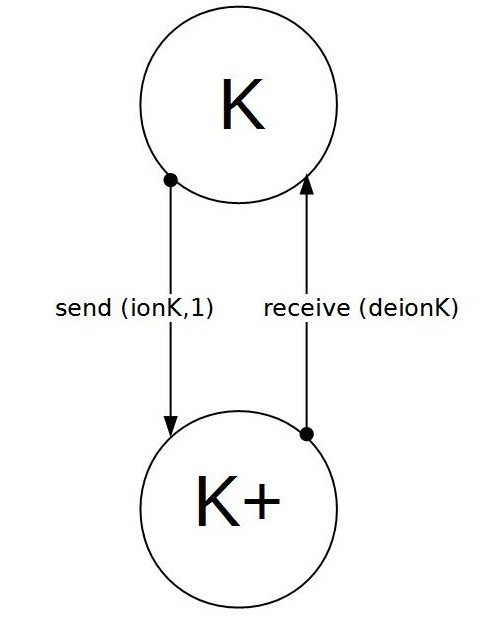
\includegraphics[width=\textwidth]{K.jpg}
    \end{subfigure}
    \begin{subfigure}[b]{0.3\textwidth}
        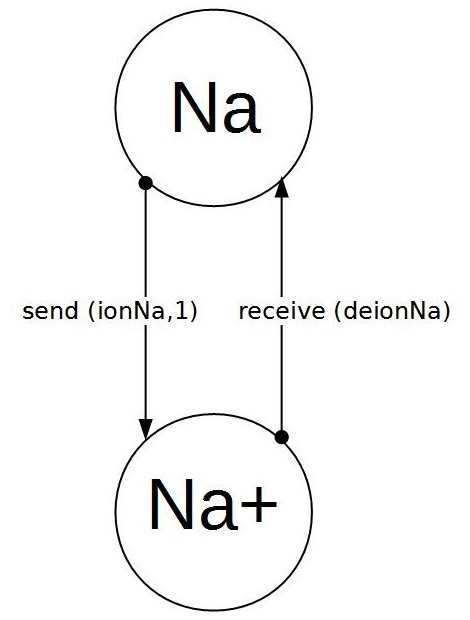
\includegraphics[width=\textwidth]{Na.jpg}
    \end{subfigure}
    \begin{subfigure}[b]{0.3\textwidth}
        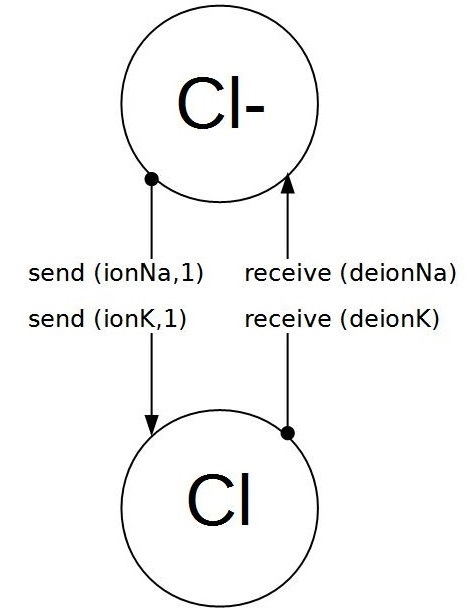
\includegraphics[width=\textwidth]{Cl.jpg}
    \end{subfigure}
\end{figure}

\tabto{0cm} {\Large \textbf{Condition with channels (example-13)}}
\vspace*{3pt}
\\
In this example, we use a condition of type if then else based on channels. First, we created the true and false value thanks to channels. We can defined those values in $\pi$-calculus : \\
$True(l) = l(t,f). \bar{t}$ \ and \ $False(l) = l(t,f). \bar{f}$
\\ Then we can create a condition by using those values.
The condition needs a channel l which corresponds to the location of a value true or false. It is defined as follow : \\
$ Cond(P,Q)(l) = (new (t,f)) \bar{l} \langle t,f \rangle .(t.P + f.Q)$
\\Depending on that the condition process will launch a different process. The processes P and Q are represented in our grammar by function which has to be spawned by the process condition. 
\newpage

\tabto{0cm} {\Large \textbf{Dining philosophers problem (example-14)}}
\vspace*{3pt}
\\
In this example, we have chosen to represent the dining philosophers problem, a recurring concurrent problem.
\begin{center}
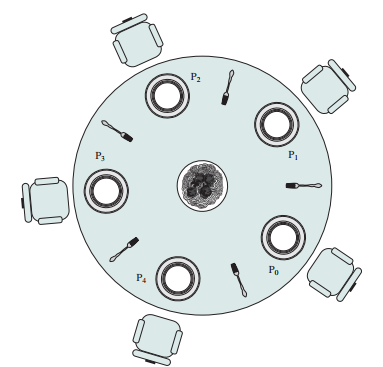
\includegraphics[scale = 0.5]{Dining.png}
\end{center}

N philosophers sit at a round table with meal plates. Forks are placed between each pair of adjacent philosophers.
\\ Each philosopher must alternately think and eat. However, a philosopher can only eat the meal when they have both left and right forks. Each fork can be held by only one philosopher and so a philosopher can use the fork only if it is not being used by another philosopher. After an individual philosopher finishes eating, they need to put down both forks so that the forks become available to others. A philosopher can take the fork on their right or the one on their left as they become available, but cannot start eating before getting both forks.

\tabto{0cm} {\Large \textbf{Whispering problem (example-15)}}
\vspace*{3pt}
\\
In this example, we have represented a situation in a bar. In this one there is a barman, customers who don't know the secret and a customer who knows the secret (There is only one secret). The barman can install 2 people at a table.  One of the 2 people will speak first, the other will listen and then both will leave the table. So, several situations are possible: \\
- the 2 people don't know the secret: they discuss and leave the table without knowing the secret \\
- one of the 2 people knows the secret and the wise man speaks first: he reveals the secret to the second person who now knows it and can spread it to other customers \\
- one of the 2 people knows the secret but the wise man doesn't speak first: the person who did not know the secret still does not know it when he leaves the table \\
- the 2 people know the secret: the person who speaks first reveals the secret but as the other person already knows it, the situation does not change, they leave the table knowing the secret.
The secret can be transmitted and spread throughout the bar.
\end{document}
